% Imporditud: tools/import_eksperimendid.py
% Allikas: Eesti füüsikaolümpiaadi eksperimendi ülesannete
%   kogu (Rael Kalda, 2023), ülesanne Ü145, lahendus L145.
\setAuthor{Koit Timpmann}
\setRound{lõppvoor}
\setYear{2014}
\setNumber{P E2}
\setDifficulty{4}
\setTopic{elektriahelad}
\setVahendid{Vooluallikas, reostaat nelja juhtmega, voltmeeter, multimeeter (ampermeetrina), hõõglamp juhtmetega, 3 juhet, 4 surveklemmi, millimeeterpaber}
\setPunktid{14}
\setAllikas{Eksperimendi kogu Ü145, lahendus lk 108}
\setLahendusseis{toores}

\prob{Elektripirni takistus}
Elektrilambi hõõgniidi takistus sõltub temperatuurist. Määrake oommeetrit kasutamata toatemperatuuril oleva hõõglambi hõõgniidi takistus.
\begin{center}
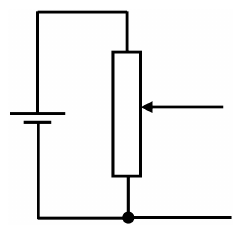
\includegraphics[width=0.25\linewidth]{2014-v3g-pe2-yl.png}
\end{center}
\textit{Vihje:} Voolutugevuse mõõtmiseks kasutage multimeetrit piirkonnaga 200 mA. Pinge reguleerimiseks kasutage reostaati potentsiomeetrilises lülituses, kus reostaadi otstele on rakendatud vooluallika pinge ning katseskeem on ühendatud reostaadi ühe otsaklemmi ja liuguri klemmiga (vt joonist). Vastavalt liuguri asendile muutub pinge katseskeemi otstel.

\hint

\solu
Katse idee ja planeerimine. Määrata lambi takistus eri-

nevatel pingetel, selleks mõõta pinge ja voolutugevus

ning arvutada seose R = U abil taksitus. JoonistaI da pinge -- takistuse graafik, pikendada graafikut pinge

väärtuseni 0 ja määrata sellele pinge väärtusele vastav

takistus. Kui pinge on 0 V, puudub lambis elektrivool ja tegemist ongi külma hõõg-

niidiga (4 p).

Vooluringi koostamine (vt joonist) (3 p).

Pinge ja voolutugevuse mõõtmine (2 p).

Tähelepanu sellele, et väikestel pingetel toimuvad mõõtmised tihedamini (1 p).

Takistuse sõltuvus voolutugevusest graafiku konstrueerimine (3 p).

Külma hõõgniidi takistuse leidmine (1 p).
\probend
